\documentclass[x11names]{article}
\usepackage{tikz}
\usepackage{pgfplots}
\usepackage{xcolor}
\usepackage{svg}
\usepackage{amsmath}
\usepackage{array}
\usepackage[skins]{tcolorbox}
\usepackage[version=4]{mhchem}
\usepackage[a4paper, total={6in, 10in}]{geometry}
%\usepackage{fouriernc}
\usepackage{xymtex}
\usepackage{textcomp}
\usepackage{eurosym}
\usepackage{mathrsfs}
\usepackage{float}
\usepackage{pst-all}
\usepackage{pst-3dplot}
\usepackage{leftindex}
\usepackage{verbatim}
\usepackage{import}
\usepackage{xifthen}
\usepackage{pdfpages}
\usepackage{transparent}
\usepackage{import}
\usepackage{pdfpages}
\usepackage{transparent}
\usepackage{amssymb}
\usepackage{hyperref}
%\usepackage{graphicx}


\definecolor{myblue}{RGB}{224, 245, 255} 
\definecolor{myred}{RGB}{234, 222, 255}
\definecolor{myorange}{RGB}{255, 102, 0}
\definecolor{egyptianblue}{RGB}{20, 52, 164}
\definecolor{neonblue}{RGB}{31, 81, 255}
\definecolor{CadmiumGreen}{RGB}{9, 121, 105}
\definecolor{BlueGreen}{RGB}{8, 143, 143}

% box
\newtcolorbox{es}[2][]{%
	enhanced,colback=white,colframe=black,coltitle=neonblue,
	sharp corners,boxrule=0.4pt,
	fonttitle=\bfseries\itshape,,
	attach boxed title to top left={yshift=-0.5\baselineskip-0.4pt,xshift=2mm},
	boxed title style={tile,size=minimal,left=0.5mm,right=0.5mm,
		colback=white,before upper=\strut},
	title=#2,#1
}

% definizioni
\newtcolorbox{blues}[2][]{%
	enhanced,colback=myblue,colframe=black,coltitle=black,
	sharp corners,boxrule=0.4pt,
	attach boxed title to top left={yshift=-0.5\baselineskip-0.4pt,xshift=2mm},
	boxed title style={tile,size=minimal,left=0.5mm,right=0.5mm,
		colback=myblue,before upper=\strut},
	title=#2,#1
}

% teoremi
\newtcolorbox{redes}[2][]{%
	enhanced,colback=myred,colframe=black,coltitle=black,
	sharp corners,boxrule=0.4pt,
	fonttitle=\itshape,
	attach boxed title to top left={yshift=-0.5\baselineskip-0.4pt,xshift=2mm},
	boxed title style={tile,size=minimal,left=0.5mm,right=0.5mm,
		colback=myred,before upper=\strut},
	title=#2,#1
}


%% regole
\renewcommand*\contentsname{Indice}
\setcounter{tocdepth}{4}
\setcounter{secnumdepth}{2}
\pgfplotsset{compat=1.15}


\usetikzlibrary{arrows}


\title{Letteratura italiana}
\author{Federico Cesari}
\date{}



\begin{document}
	
	\begin{titlepage}
	\begin{center}
		\vspace*{1cm}
		
		\textbf{\LARGE Relazione di laboratorio - Pendolo semplice}
		
		\vspace{0.3cm}
		\large \textit{Misura del periodo di un pendolo semplice} \\
		
		\vspace{0.5cm}
		\Large Federico Cesari \\
		
		\small 1096759 
		\vspace{0.2cm}
		
		\small Gruppo 5
		
		
		\vspace{3cm}
		\begin{center}
			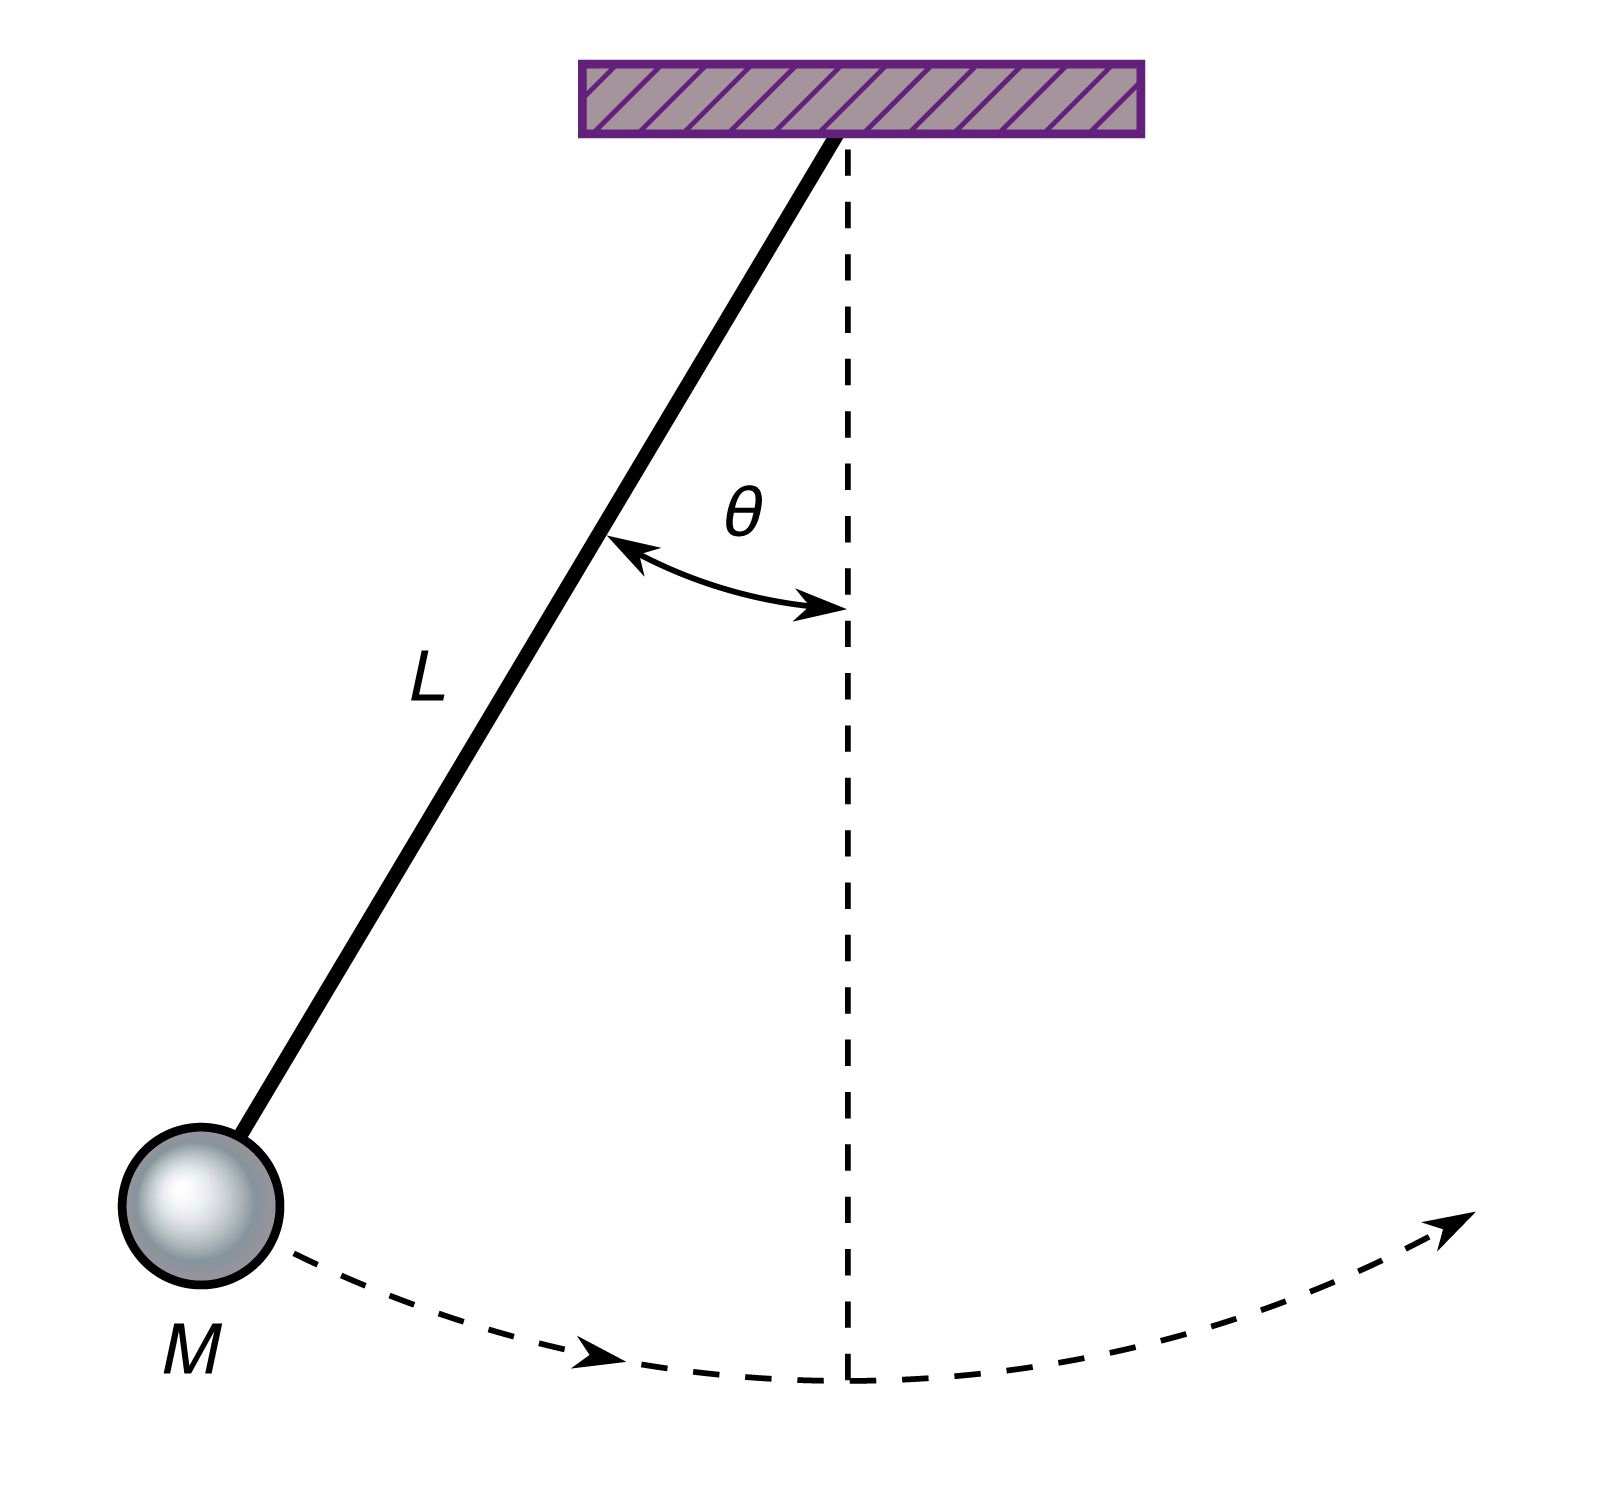
\includegraphics[scale=0.1]{IMG_0200.jpeg}	
		\end{center}
		
		
		
		\vfill
		
		
		
		corso A\\
		Università degli studi di Torino, Torino\\
		4 aprile 2024\\
		
		
	\end{center}
\end{titlepage}
	\tableofcontents
	\newpage
	
	
	\section{Serie numeriche}
	Sia \(a_{n} \subset \mathbb{C}\) successione di numeri complessi, chiamiamo \textbf{serie numerica} la sommatoria 
	\[ 
	\sum_{n=0}^{\infty} a_{n} = a_{1} + \dots + a_{n} + \dots
	\]
	Chiamiamo invece \textbf{ridotta ennesima} della serie la quantità
	\[ 
	S_{N} = \sum_{n=0}^{N} a_{n} = a_{1} + \dots + a_{N} \qquad N \in \mathbb{N}
	\]
	Abbiamo costruito la \textbf{successione delle ridotte} \(S_{N}\) con \(N\in\mathbb{N}\).
	
	\subsection{Successioni di numeri complessi}
	\begin{center}
		\fboxsep11pt
		\colorbox{myblue}{\begin{minipage}{5.75in}
				\begin{blues}{Definizione: Serie convergente divergente e indeterminata}
					Se il limite 
					\[ 
					\lim_{N\to\infty}S_{N} = S \in \mathbb{C}
					\]
					diciamo che la serie 
					\[ 
					\sum_{n=0}^{\infty} a_{n} = S
					\]
					converge ad \(S\) e chiamiamo \(S\) somma della serie. \\
					
					Nel caso in cui \(S_{N}\) sia divergente o indeterminata la serie è divergente o indeterminata.
				\end{blues}
		\end{minipage}}       
	\end{center}
	
	
	\subsection{Carattere di una serie}
	Si osserva che preso \(n_{0} \in \mathbb{N}\) e considerando la serie
	\[ 
	\sum_{n=n_{0}}^{\infty} a_{n} \quad \text{questa ha lo stesso carattere di }\quad \sum_{n=0}^{\infty} a_{n}
	\]
	Chiaramente la somma sarà diversa, il carattere tuttavia non cambia.
	\begin{center}
		\fboxsep11pt
		\colorbox{myred}{\begin{minipage}{5.75in}
				\begin{redes}{}
					\subsubsection{Teorema: Condizione necessaria di convergenza}
					Sia \(a_{n} \subset \mathbb{C}\). Condizione necessaria affinché la serie
					\[ 
					\sum_{n=0}^{\infty} a_{n}
					\]
					converga è che 
					\[ 
					\lim_{n\to \infty} a_{n} = 0
					\]
				\end{redes}
		\end{minipage}}        
	\end{center}
	
	\begin{es}{Dimostrazione}
		Supponiamo che 
		\[
		\lim_{n\to\infty}S_N = S \in \mathbb{C} \qquad a_n = S_n - S_{n-1}
		\]
		allora
		\[
		\lim_{n\to\infty} a_n = \lim_{n\to\infty} S_n - S_{n-1} = S - S = 0 
		\]
	\end{es}
	
	\begin{center}
		\fboxsep11pt
		\colorbox{myred}{\begin{minipage}{5.75in}
				\begin{redes}{}
					\subsubsection{Teorema: "Linearità delle serie"}
					Prendiamo due serie di numeri complessi convergenti rispettivamente ad \(A\) e a \(B\):
					\[ 
					sum_{n=0}^{\infty} a_{n} = A \qquad\qquad sum_{n=0}^{\infty} b_{n} = B
					\]
					allora
					\[ 
					i) \qquad \forall \; \lambda \in \mathbb{C} \quad  \sum_{n=0}^{\infty} \lambda a_{n} = \lambda \sum_{n=0}^{\infty}  a_{n}= \lambda A
					\]
					\[ 
					ii) \qquad \sum_{n=0}^{\infty}  (a_{n} + b_{n} )= \sum_{n=0}^{\infty} a_{n} + \sum_{n=0}^{\infty} b_{n} = A + B
					\]
				\end{redes}
		\end{minipage}}        
	\end{center}
	
	\subsection{Serie geometrica, serie telescopiche e armoniche}
	\subsubsection{Serie geometrica}
	Fissato \(q \in \mathbb{C}\) si dice \textbf{serie geometrica} di ragione \(q\) la serie
	\[ 
	\sum_{n=0}^{\infty} q^n = \frac{1-q^{N+1}}{1-q}
	\]
	il carattere è determinato da \(q\):
	\[ 
	\begin{array}{lc}
		|q| < 1 & \text{la serie converge} \\
		|q| > 1 \text{ o } q = 1 & \text{la serie diverge} \\
		|q| = 1 \text{ e } q \neq 1 & \text{la serie è indeterminata} \\
	\end{array}
	\] \\
	
	\begin{es}{Dimostrazione}
		\begin{enumerate}
			\item $|q| < 1$\\
			\[ 
			S_N = \sum_{n=0}^{N} q^n = \frac{1-q^{N+1}}{1-q}
			\]
			
			Verifichiamo che $S_N$ sia effettivamente uguale a quanto scritto:
			
			\begin{align*}
				(1-q)\sum_{n=0}^{N} q^n &= \sum_{n=0}^{N} q^n \;-\; q\sum_{n=0}^{N} q^n \\
				&= \sum_{n=0}^{N} q^n \;-\; \sum_{n=0}^{N} q^{n+1} \\ 
				&= 1 \,-\, q^{N+1}
			\end{align*}
			
			Allora: 
			
			\[ 
			|q^{N+1}| = |q|^{N+1} \to 0 \;\; \text{per} \;\; N \to +\infty
			\]
			
			\[
			\Longrightarrow \lim_{N\to \infty} q^{N+1} = 0
			\]
			\end{enumerate}
			\end{es}
			\begin{es}{}
			Dunque: 
			\[
			\lim_{n\to \infty} S_N \;= \;\lim_{n\to \infty} \frac{1-q^{N+1}}{1-q} \;=\; \frac{1}{1-q}\cdot \lim_{n\to \infty} (1-q^{N+1}) \;=\; \frac{1}{1-q}
			\]
			\begin{enumerate}
				\setcounter{enumi}{1}
			\item $|q| > 1$\\
			
			Usando la disuguaglianza triangolare inversa si ha: 
			\[
			|S_N| = \left|\frac{1-q^{N+1}}{1-q}\right| = \frac{|1-q^{N+1|}}{|1-q|} \geq 
			\frac{|1|-|q^{N+1}|}{|1-q|}
			\]
			
			Da cui segue: 
			
			\begin{align*}
				\lim_{N\to \infty} \frac{|1|-|q^{N+1}|}{|1-q|} &=\; \frac{1}{|1-q|} \lim_{N\to \infty} \left|1-|q|^{N+1}\right| \\
				&=\; \frac{1}{|1-q|} \left| 1 - \lim_{N\to \infty}|q|^{N+1}\right| \\ 
				&= +\infty
			\end{align*}
			
			\item $q = 1$
			\[
			S_N = \sum_{n=0}^{N} 1 = 1 + 1 + ... + 1 = N + 1
			\]
			
			\[
			\Longrightarrow \quad \lim_{N \to \infty} S_N = +\infty \quad \Longrightarrow \quad\text{La serie è divergente}
			\]
			
		\end{enumerate}
		
	\end{es}
	
	\subsubsection{Serie telescopiche}
	Chiamiamo \textbf{serie telescopiche} le seguenti le serie di forma
	\[ 
	a_{0} + \sum_{n=1}^{\infty} (a_{n} - a_{n-1}) \qquad a_{n} \subset \mathbb{C}
	\]
	\begin{es}{\textcolor{black}{alcuni esempi di serie telescopiche}}
		\begin{minipage}{0.5\textwidth}
			\[ 
			i) \qquad \sum_{n=1}^{\infty} \frac{1}{n(n+1)} = 1
			\]
		\end{minipage}
		\begin{minipage}{0.5\textwidth}
			\[ 
			ii) \qquad \sum_{n=1}^{\infty} \log\left(1 + \frac{1}{n}\right) = +\infty
			\]
		\end{minipage}
	\end{es}
	
	\subsubsection{Serie armonica}
	Prende il nome di \textbf{serie armonica generalizzata}
	\[ 
	\sum_{n=1}^\infty \frac{1}{n^a}
	\]
	Il carattere è terminato da \(a\):
	\[ 
	\begin{array}{lc}
		a \leq 1 & \text{la serie diverge} \\
		a > 1  & \text{la serie converge} \\
	\end{array}
	\] \\
	
	\noindent
	Mostriamo perché la serie con \(a=1\) diverge:
	\[ 
	a_{n} = \frac{1}{n} \to 0, \quad n \to \infty
	\]
	\[ 
	\log\left(1+\frac{1}{n}\right) \approx \frac{1}{n}, \quad n \to \infty
	\]
	\[ 
	\sum \log\left(1+\frac{1}{n}\right) \text{ diverge }\quad \Longrightarrow \quad\sum \frac{1}{n} \text{ diverge per il criterio del confronto asintotico.}
	\] \\
	
	\begin{es}{Dimostrazione}
		\begin{enumerate}
			\item \(a\leq 1\) con \(a \in \mathbb{R}\) così che valga \(\frac{1}{n^a} \geq \frac{1}{n}\) \(\forall n \geq 1\).
			
			\[ 
			\sum_{n=1}^\infty\frac{1}{n^a} \geq \sum_{n=1}^\infty\frac{1}{n} \quad \text{serie armonica divergente}
			\]
			quindi per il criterio del confronto, essendo maggiore di una serie divergente, diverge anche la serie \(\sum\frac{1}{n^a}\). \\
			
			\item $a > 1$\\
			
			In generale vale:
			\[
			\frac{1}{n^{\alpha}} \; \leq \; \int_{n-1}^{n} \frac{dx}{x^{\alpha}}
			\] \\
			Allora: 
			\[
			S_n = \sum_{n=2}^{n} \frac{1}{n^{\alpha}} \leq \int_{1}^{n}\frac{dx}{x^{\alpha}} \leq\int_{1}^{\infty}\frac{dx}{x^{\alpha}}
			\]
			Si ha inoltre: 
			\begin{align*}
				\int_{1}^{\infty}\frac{1}{x^{\alpha}}dx &= \left[\frac{x^{-\alpha+1}}{-\alpha+1}\right]^{\infty}_{1}\\
				&=\left[\frac{1}{(-\alpha+1)x^{\alpha-1}}\right]^{\infty}_{1}\\
				&=\frac{1}{\alpha-1}<\infty
			\end{align*}
			
			$\{S_n\}$ è monotona crescente e superiormente limitata $\Longrightarrow$ la serie converge 
		\end{enumerate}
	\end{es}
	\subsection{Serie a termini non negativie a segni alterni}
	
	\[ 
	\text{Termini non negativi} \qquad \sum_{n=0}^{\infty} a_{n}, \qquad a_{n} \geq 0, \qquad \forall n \in \mathbb{N}
	\]
	\[ 
	\text{Segni alterni} \quad \qquad \sum_{n=0}^{\infty} (-1)^nb_{n}, \qquad b_{n} > 0, \qquad \forall n \in \mathbb{N}
	\]
	\begin{center}
		\fboxsep11pt
		\colorbox{myred}{\begin{minipage}{5.75in}
				\begin{redes}{}
					\subsubsection{Teorema: Le serie a termini non negativi o convergono o divergono}
					Sia \(\sum_{n=0}^\infty a_{n}\) una serie a termini non negativi, questa può o convergere o divergere, non può essere indeterminata.
				\end{redes}
		\end{minipage}}        
	\end{center}
	\begin{es}{Dimostrazione}
		Prendo \(\{S_{N}\}_{N\in\mathbb{N}}\) \textbf{monotona crescente}:
		\[ 
		S_{N+1} = S_{N} + a_{N+1} \geq S_{N}
		\]
		Se il limite converge a \(S\) limite superiore 
		\[ 
		\lim_{N\to\infty} S_{N} = S \in [0,+\infty)  \qquad S = \text{sup }_{N\in\mathbb{N}} S_{N}
		\]
		\[ 
		\Longrightarrow \text{ La serie converge}
		\]
		Se \(\{S_{N}\}_{N\in\mathbb{N}}\) non è superiormente limitata si ha 
		\[ 
		\lim_{N\to\infty} S_{N} = +\infty
		\]
		\[ 
		\Longrightarrow \text{ La serie diverge}
		\]
		
	\end{es}
	
	\begin{center}
		\fboxsep11pt
		\colorbox{myblue}{\begin{minipage}{5.75in}
				\begin{blues}{Definizione: Convergenza assoluta}
					Sata una serie di numeri complessi \(\sum_{n=0}^{\infty} a_{n} \in \mathbb{C}\) si dice che la serie è \textbf{assolutamente convergente} se è convergente la serie
					\[ 
					\sum_{n=0}^{\infty} |a_{n}|
					\]
				\end{blues}
		\end{minipage}}       
	\end{center}
	\begin{center}
		\fboxsep11pt
		\colorbox{myred}{\begin{minipage}{5.75in}
				\begin{redes}{}
					\subsubsection{Teorema: Convergenza assoluta implica convergenza semplice}
					Sia \(\sum_{n=0}^{\infty} a_{n} \subset \mathbb{C}\). Supponiamo che la serie sia assolutamente convergente, allora la serie è anche semplicemente convergente. Inoltre vale
					\[ 
					\left|\sum_{n=0}^{\infty} a_{n}\right| \leq \sum_{n=0}^{\infty} |a_{n}|
					\]
				\end{redes}
		\end{minipage}}        
	\end{center}
	
	\subsection{Criteri applicabili alle serie}
	
	\subsubsection{Criterio del confronto}
	Siano  $\sum_{n=0}^{\infty}a_n$ e $\sum_{n=0}^{\infty}b_n$ due serie a termini positivi. \\
	Supponiamo che esiste finito $n_0 \in \mathbb{N}$ t.c. 
	\[ 
	\begin{array}{ll}
		a_n \leq b_n \quad,\quad \forall n \geq n_0
	\end{array}
	\]
	Allora: \\
	
	1) se $\sum_{n=0}^{\infty}b_n$ è convergente $\Longrightarrow$ $\sum_{n=0}^{\infty}a_n$ è convergente\\
	
	2) se $\sum_{n=0}^{\infty}a_n$ è divergente $\Longrightarrow$ $\sum_{n=0}^{\infty}b_n$ è divergente \\
	
	\begin{es}{Dimostrazione}
		Non è restrittivo supporre $n_0 = 0$. \\
		
		1) $S_N \quad = \quad \sum_{n=0}^{N}a_n \quad\leq\quad  \sum_{n=0}^{N}b_n \quad\leq\quad  \sum_{n=0}^{\infty}b_n \quad < \quad \infty$ \\
		
		$S_N$ è una successione monotona crescente superiormente limitata $\Longrightarrow$ è convergente \\
		
		2) Per \textbf{contraddizione}, supponiamo che: \\
		
		$\sum_{n=0}^{\infty}b_n$ converga $\Longrightarrow$ per il punto 1) la serie  $\sum_{n=0}^{\infty}a_n$ dovrebbe convergere. \\ Abbiamo ottenuto una contraddizione. \\
		
		Dunque:
		\begin{center}
			$\Longrightarrow$  $\sum_{n=0}^{\infty}b_n$ diverge.
		\end{center}
		
	\end{es}
	
	\subsubsection{Criterio del confronto asintotico}
	\subsubsection{Criterio della radice} 
	Sia \(\sum a_{n}\) serie a termini positivi. Supponiamo che esista
	\[ 
	\lim_{n\to \infty} \sqrt[n]{a_{n}} = \lim a^{1/n}_{n} = l \in [0,+\infty]
	\]
	allora 
	\[ 
	\begin{array}{ll}
		l<1 & \text{la serie converge} \\
		l>1 & \text{la serie diverge} \\
		l=1 & \text{caso dubbio}
	\end{array}
	\]
	\subsubsection{Criterio del rapporto} 
	Sia \(\sum a_{n}\) serie a termini positivi. Supponiamo \(a_{n} > 0 \forall n\) e che esista
	\[ 
	\lim_{n\to \infty} \frac{a_{n+1}}{a_{n}} =  l \in [0,+\infty]
	\]
	allora 
	\[ 
	\begin{array}{ll}
		l<1 & \text{la serie converge} \\
		l>1 & \text{la serie diverge} \\
		l=1 & \text{caso dubbio}
	\end{array}
	\]
	\subsubsection{Criterio dell'integrale di Mc. Laurin}
	\subsubsection{Criterio di Leibniz} 
	Sia data la serie \(\sum_{n=0}^{\infty}(-1)^n b_{n}\) con \(b_{n} > 0 \forall n\). Supponiamo
	\[ 
	\begin{array}{l}
		1) \qquad b_{n+1} \leq b_{n} \quad \forall n \qquad \text{(la serie è decrescente)} \\
		2) \qquad \lim_{n\to\infty} b_{n} = 0
	\end{array}
	\]
	Allora la serie converge a 
	\[ 
	S = \sum_{n=0}^{\infty}(-1)^nb_{n}
	\]
	e \(|S - S_{N}| \leq b_{N+1} \quad \forall N \in \mathbb{N}\).
	
	
	\begin{es}{}
		\subsection{Procedimento per la risoluzione degli esercizi}
		\begin{enumerate}
			\item Verificare la condizione necessaria di convergenza
			\item Se è a \textbf{valori non negativi}: 
			\begin{enumerate}
				\item Tramite confronto e confronto asintotico verificare se questa converge o diverge.
			\end{enumerate}
			\item Se è a \textbf{segni alterni}:
			\begin{enumerate}
				\item Ne studio il modulo;
				\item Tramite confronto e confronto asintotico verificare se questa converge o diverge assolutamente;
				\item Se diverge uso il \textbf{criterio di Leibniz};
				\item Verifico che sia strettamente decrescente;
				\item Se lo è la serie è semplicemente convergente.
			\end{enumerate}
		\end{enumerate}
	\end{es}
	
	\newpage
	\section{Topologia di \(\mathbb{R}^n\)}
	Questa sezione contiene solo definizioni, non sto a distinguerle con il riquadro colorato.
	
	\subsubsection*{Intorno}
	Si dice \textbf{intorno sferico} di centro \(x_{0} \in \mathbb{R}^n\) e raggio \(r>0\) l'insieme
	\[ 
	B(x_{0},r) = \{x \in \mathbb{R}^n \quad |\quad d(x,x_{0}) = |x-x_{0}| < r\}
	\]
	La distanza dalle due dimensioni in poi chiaramente è espressa come
	\[ 
	d(x,x_{0}) = \sqrt{(x-x_{0})^2 + (y-y_{0})^2 + \dots }
	\]
	
	
	\subsubsection*{Punto di accumulazione}
	Sia \(A \subseteq \mathbb{R}^n\) e \(x_{0} \in \mathbb{R}^n\). Si dice \textbf{punto di accumulazione} per \(A\) se
	\[ 
	\forall r > 0 \qquad \left(B(x_{0},r) \smallsetminus \{x_{0}\} \right) \cap A \neq \varnothing
	\]
	\textit{In sostanza è un punto di accumulazione se ogni suo intorno contiene punti di \(A\) diversi da se stesso}
	\subsubsection*{Insieme limitato}
	\(A \subseteq \mathbb{R}^n\) si dice limitato se
	\[ 
	\exists M > 0 \quad | \quad \|x\| \leq M, \quad \forall x \in A
	\]
	\[ 
	A \subseteq \overline{B(O,M)} \quad \text{con} \quad B(O,M) = \{x \in \mathbb{R} \quad | \quad \|x\|\leq M \}
	\]
	\subsubsection*{Insieme aperto}
	\(A\subseteq \mathbb{R}^n\) si dice aperto se 
	\[ 
	\forall x \in A \quad \exists r > 0 \quad | \quad B(x_{o},r) \subset A
	\]
	\begin{itemize}
		\item	\(\mathbb{R}^n\) è un insieme aperto;
		\item   L'intersezione di qualunque famigia di un chiuso è un aperto,
		\item   L'unione di un numero finito di chiusi è un aperto.
	\end{itemize}
	
	\subsubsection*{Insieme chiuso}
	\(C\subseteq \mathbb{R}^n\) si dice \textbf{chiuso} se il suo complementare \(\mathbb{R}^n \backslash C\) è un aperto.
	
	\begin{itemize}
		\item	Sono chiusi gli insiemi \(\mathbb{R}^n\) e \(\varnothing\);
		\item  l'intersezione di qualunque famigia di un chiuso è un chiuso;
		\item   l'unione di un numero finito di chiusi è un chiuso.
	\end{itemize}
	
	
	\subsubsection*{Insieme compatto}
	Un sottoinsieme \(K\subset \mathbb{R}^n\) è detto \textbf{compatto} se è chiuso e limitato.
	
	\subsubsection*{Putni interni, esterni e di frontiera}
	\[ 
	\text{Interno:} \qquad \exists r > 0 \quad | \quad B(x_{0}, r) \subset A
	\]
	\[ 
	\text{Interno:} \qquad \exists r > 0 \quad | \quad B(x_{0}, r) \cap A = \varnothing
	\]
	Se \(x_{0}\) non è né interno né esterno è un putno di frontiera.
	
	\begin{itemize}
		\item	\(Int(A)\) è un aperto ed è il più grande aperto contenuto in \(A\);
		\item   \(Int(A) \cap Fr(A)\) è un chiuso ed è il più piccolo chiuso contenente \(A\) e viene denotato con \(\bar{A}\);
		\item   \(Fr(A)\) è un chiuso;
		\item \(A\) è chiuso \(\Longleftrightarrow\) \(A = Int(A)\);
	\end{itemize}
	
	
	% Continuità per campi scalari
	
	\section{Limiti di funzioni in più variabili}
	
	\begin{center}
		\fboxsep11pt
		\colorbox{myblue}{\begin{minipage}{5.75in}
				\begin{blues}{Definizione: Limite di funzione a più variabili}
					Sia $F:A\subseteq\mathbb{R}^n \to \mathbb{R}^m.$\\
					
					Sia $x_0 \in \mathbb{R}^n$ punto di accumulazione per $A$.\\
					
					Diciamo che $l \in \mathbb{R}^m$ è limite di $F$ per $x\to x_0$ e scriviamo $\lim_{x\to x_0}F(x) = l \quad\text{se:}$
					
					\[
					\forall\; \epsilon > 0\;,\; \exists\; \delta > 0\;\;|\;\;\forall\,x \in A\;,\; 0 < \|x-x_0\| < \delta \Longrightarrow \|F(x)-l\|<\epsilon
					\]
				\end{blues}
		\end{minipage}}       
	\end{center}
	
	\begin{center}
		\fboxsep11pt
		\colorbox{myred}{\begin{minipage}{5.75in}
				\begin{redes}{}
					\subsubsection{Teorema: Equivalenza tra limite globale e limite componente per componente}
					Sia $F:A\subseteq\mathbb{R}^n \to \mathbb{R}^m.$\\
					
					Sia $x_0 \in \mathbb{R}^n$ punto di accumulazione per $A$ ed $F(x) = (F_1(x),...,F_m(x)).$\\
					
					Allora, preso $l \in \mathbb{R}^m$ si ha: \\
					\[
					\lim_{x\to x_0} F(x) = l \; \Longleftrightarrow \; \lim_{x\to x_0} F_j(x)=l_j \quad \forall\,j=1,...,m
					\]
				\end{redes}
		\end{minipage}}
	\end{center}
	
	\begin{es}{Dimostrazione} 
		\begin{itemize}
			\item $\Longrightarrow$ Supponiamo $\lim_{x \to x_0} F(x) = l$, allora: 
			\[
			\forall\; \epsilon > 0\;,\; \exists\; \delta > 0\;\;|\;\;\forall\,x \in A\;,\; 0 < \|x-x_0\| < \delta \Longrightarrow \|F(x)-l\|<\epsilon
			\]
			Segue che: 
			\[
			\left|F_j(x)-l_j\right|=\sqrt{\left(F_j(x)-l_j\right)^2}\,\leq\,\sqrt{\left(F_j(x)-l_j\right)^2+...+\left(F_m(x)-l_m\right)^2} = \|F(x)-l\|<\epsilon
			\]
			\[
			\centering{\color{CadmiumGreen} \forall\,j=1,...,m}
			\]
			
			\[
			\Longrightarrow \left|F_j(x)-l_j\right| < \epsilon\,,\quad\forall\,x\in A\; |\; 0 < \|x-x_0\| < \delta 
			\] \\
			\item $\Longleftarrow$ Supponiamo $\lim_{x \to x_0} F_j(x) = l_j\,,\,{\color{CadmiumGreen}\forall \,j=1,...,m}$
			\[ 
			\forall\; \epsilon > 0\;,\; \exists\; \delta > 0\;\;|\;\;\forall\,x \in A\;,\; 0 < \|x-x_0\| < \delta \Longrightarrow \|F_j(x)-l_j\|<\frac{\epsilon}{\sqrt{m}} \quad {\color{CadmiumGreen} \forall \,j=1,...,m}
			\]
			
			\[\text{Dove abbiamo preso arbitrariamente  } \epsilon = \frac{\epsilon}{\sqrt{m}} \]
			
			\[
			\|F(x)-l\|^2 = \left(F_1(x)-l_1\right)^2+...+\left(F_m(x)-l_m\right)^2 < \frac{\epsilon^2}{m} + ... + \frac{\epsilon^2}{m} = \epsilon^2
			\]
			
			\[
			\forall\,x\in A\;\; |\;\; 0 < \|x-x_0\| < \delta \quad\text{dove}\quad\delta = min\{\delta_1,...,\delta_m\}
			\]
			
			Quindi: 
			\[
			\|F(x)-l\| < \epsilon
			\]
			
		\end{itemize}
	\end{es}
	
	\paragraph{Punto all'infinito}
	In dimensioni maggiori di 1 non si può più distinguere tra \(+\infty\) e \(-\infty\), allora si parla solo di \textbf{punto all'infinito}
	
	\subsection{Utilizzo delle curve}
	
	\begin{center}
		\fboxsep11pt
		\colorbox{myred}{\begin{minipage}{5.75in}
				\begin{redes}{}
					\subsubsection{Proprietà}
					Sia \(f:A\subseteq \mathbb{R}^n \to \mathbb{R}\), \(\boldsymbol{x_{0}} \in \mathbb{R}^n\) punto di accumulazione per \(A\). Supponiamo che esista il limite
					\[ 
					\lim_{\boldsymbol{x}\to\boldsymbol{x_0}}f(\boldsymbol{x}) = l
					\]
					Allora presa una qualunque curva passante per \(x_{0}\) e con sostegno in \(A \cup \{\boldsymbol{x_{0}}\}\), ovvero 
					\[
					\boldsymbol{\gamma}: I \to A\cup\{\boldsymbol{x_{0}}\} \;\ \text{t.c.} \;\ \exists  t_{0} \in I, \;\ \boldsymbol{\gamma}(t_{0}) = \boldsymbol{x_{0}}
					\]
					si ha
					\[ 
					\lim_{t\to t_0}f(\boldsymbol{\gamma}(t)) = l
					\]
				\end{redes}
		\end{minipage}}
	\end{center}
	
	\paragraph{Corollario} Sia \(f:A\subseteq \mathbb{R}^n \to \mathbb{R}\), \(\boldsymbol{x_{0}} \in \mathbb{R}^n\) punto di accumulazione per \(A\).
	\begin{enumerate}
		\item Se esiste una curva
		\[ 
		\boldsymbol{\gamma}: I \to A\cup\{\boldsymbol{x_{0}}\} \;\ \text{t.c.} \;\ \exists  t_{0} \in I, \;\ \boldsymbol{\gamma}(t_{0}) = \boldsymbol{x_{0}}
		\]
		e 
		\[ 
		\nexists \lim_{t\to t_0}f(\boldsymbol{\gamma}(t))
		\]
		allora
		\[ 
		\nexists \lim_{\boldsymbol{x}\to \boldsymbol{x_{0}}}f(\boldsymbol{\boldsymbol{x}})
		\]
		\item Se esistono due curve
		\[ 
		\boldsymbol{\gamma}_{1}, \boldsymbol{\gamma}_{2} \;\ \text{t.c.} \;\ \boldsymbol{\gamma}_{1}(t_{0}) = \boldsymbol{\gamma}_{2}(t'_{0}) = \boldsymbol{x_{0}}
		\]
		e
		\[ 
		\begin{array}{c}
			\lim_{t\to t_0}f(\boldsymbol{\gamma}(t)) = l_{1} \\
			\lim_{t\to t'_0}f(\boldsymbol{\gamma}(t)) = l_{2}
		\end{array} \qquad \text{t.c.} l_{1} \neq l_{2}
		\]
		allora
		\[ 
		\nexists \lim_{\boldsymbol{x}\to \boldsymbol{x_{0}}}f(\boldsymbol{\boldsymbol{x}})
		\]
	\end{enumerate}
	
	\subsection{Punti stazionari per campi scalari e vettoriali}
	\begin{center}
		\fboxsep11pt
		\colorbox{myred}{\begin{minipage}{5.75in}
				\begin{redes}{}
					\subsubsection{\textbf{Teorema di Weierstra{\ss}}}
					Sia \(f:K\subset \mathbb{R}^n \to \mathbb{R}\) con \(k\neq \varnothing\) e compatto.
					
					Se \(f\) è continua su \(K\) allora ammette un massimo su \(K\).
				\end{redes}
		\end{minipage}}
	\end{center}
	
	\begin{center}
		\fboxsep11pt
		\colorbox{myblue}{\begin{minipage}{5.75in}
				\begin{blues}{Definizione: Continuità}
					Sia $f:A \subseteq\mathbb{R}^n\to \mathbb{R}^m$  e sia \(\boldsymbol{x_{0}} \in A\).
					
					\(f\) si dice continua in \(x_{0}\) se 
					\[ 
					\forall \varepsilon  > 0 \quad \exists \delta > 0 \quad | \quad \forall \boldsymbol{x_{0}} \in A, \quad \|x-x_{0}\| < \delta \quad \Longrightarrow \quad \|f(\boldsymbol{x}) - f(\boldsymbol{x_{0}})\| < \varepsilon
					\]
					
					Inoltre se \(\boldsymbol{x_{0}} \in A\) è punto di accumulazione per \(A\), allora dalla definizione di limite otteniamo 
					\[ 
					f \;\ \text{continua in } \boldsymbol{x_{0}} \quad \Longleftrightarrow \quad \lim_{\boldsymbol{x}\to \boldsymbol{x_{0}}} f(\boldsymbol{x}) = f(\boldsymbol{x_{0}})
					\]
				\end{blues}
		\end{minipage}}       
	\end{center}
	
	\begin{center}
		\fboxsep11pt
		\colorbox{myblue}{\begin{minipage}{5.75in}
				\begin{blues}{Definizione: Uniformemente continua}
					Sia \(f:A\subseteq \mathbb{R}^n  \to \mathbb{R}\), \(f\) si dice uniformemente continua su \(A\) se
					\[ 
					\forall \varepsilon  > 0 \quad \exists \delta > 0 \quad | \quad \forall x,y \in A, \quad \|x-y\| < \delta
					\]
					allora 
					\[ 
					|f(x) - f(y)| < \varepsilon
					\] \\
					
					Vale 
					\[ 
					f \text{ unif. cont. su } A \Longleftrightarrow f \text{ continua su } A
					\]
				\end{blues}
		\end{minipage}}       
	\end{center}
	
	\begin{center}
		\fboxsep11pt
		\colorbox{myblue}{\begin{minipage}{5.75in}
				\begin{blues}{Definizione: Punto stazionario}
					Sia $A \subseteq\mathbb{R}^n, A$ aperto, $f:A\to\mathbb{R}, \;f\in\mathbb{C}^1(A).$ Sia $\boldsymbol{\bar{x}}\in A$. Si dice che $\boldsymbol{\bar{x}}$ è un punto stazionario (o critico) se: 
					\[\nabla f(\boldsymbol{\bar{x}})=0\]
				\end{blues}
		\end{minipage}}       
	\end{center}
	
	\begin{center}
		\fboxsep11pt
		\colorbox{myblue}{\begin{minipage}{5.75in}
				\begin{blues}{Definizione: Massimi e Minimi}
					Sia $f:A\subseteq\mathbb{R}^n\to \mathbb{R}$, $A$ sottoinsieme qualunque. Si dice che $\boldsymbol{\bar{x}}\in A$ è: 
					\begin{enumerate}
						\item Punto di minimo locale per f se: $\exists\, r>0\;|\;f(x)\geq f(\boldsymbol{\bar{x}}), \forall\,x\in B(\boldsymbol{\bar{x}},r) \cap Dom\,f$
						\item  Punto di minimo locale per f se: $\exists\, r>0\;|\;f(x)\leq f(\boldsymbol{\bar{x}}), \forall\,x\in B(\boldsymbol{\bar{x}},r) \cap Dom\,f$
					\end{enumerate}
					In particolare, se la condizione 1) o 2) valgono $\forall\,x\in Dom\,f \Longrightarrow \boldsymbol{\bar{x}}$ si dice punto di minimo/massimo globale per f. 
				\end{blues}
		\end{minipage}}       
	\end{center}
	
	\begin{center}
		\fboxsep11pt
		\colorbox{myblue}{\begin{minipage}{5.75in}
				\begin{blues}{Definizione: Punti di sella}
					Sia $A$ aperto, $f:A\to \mathbb{R},\;f\in\mathbb{C}^1(A)$. Se $\boldsymbol{\bar{x}}\in A$ è un punto stazionario ($\nabla f(\boldsymbol{\bar{x}})=0$) e non è un punto di massimo o di minimo locale, allora si dice punto di sella. 
				\end{blues}
		\end{minipage}}       
	\end{center}
	
	
	\begin{center}
		\fboxsep11pt
		\colorbox{myred}{\begin{minipage}{5.75in}
				\begin{redes}{}
					\subsubsection{\textbf{Teorema di Fermat}}
					Sia \(A\subseteq \mathbb{R}^n\) aperto, \(f:A\subseteq \mathbb{R}^n \to \mathbb{R}\) con \(f\in\mathcal{C}^1(A)\). 
					
					Se \(\boldsymbol{\bar{x}} \in A\) è un punto di minimo/massimo locale, allora
					\[ 
					\nabla f(\boldsymbol{\bar{x}}) = 0
					\]
					\(\boldsymbol{\bar{x}}\) è un punto stazionario.
				\end{redes}
		\end{minipage}}
	\end{center}
	\begin{es}{Dimostrazione}
		Ci riconduciamo al teorema di Fermat per funzioni di una variabile.
		
		Sia \(\boldsymbol{\bar{x}} = (\bar{x}_{1},\dots,\bar{x}_{n})\) punto  di minimo locale:
		\[ 
		\exists \,r> 0 \quad | \quad B(\boldsymbol{\bar{x}},r) \subset A \quad \text{e} \quad f(\boldsymbol{x}) \geq f(\boldsymbol{\bar{x}}), \quad {\color{CadmiumGreen}\forall\, \boldsymbol{x} \in B(\boldsymbol{\bar{x}},r)}
		\]
		quindi si può dire anche che
		\[ 
		x = \boldsymbol{\bar{x}} + \boldsymbol{h} \quad \Longleftrightarrow \quad f(\boldsymbol{\bar{x}} + \boldsymbol{h}) \geq f(\boldsymbol{\bar{x}}),\qquad {\color{CadmiumGreen}\forall\, \boldsymbol{h} \;\, t.c. \;\, \|\boldsymbol{h}\| < r}
		\]
		
		Definiamo ora una funzione \(g\)
		\[
		g(x_{1}) = f(x_{1},\bar{x}_{2},\dots,\bar{x}_{n})
		\]
		
		Se \(\boxed{n=2}\)
		\[ 
		g: (\bar{x}_{1} -r, \bar{x}_{1}+r) \to \mathbb{R}
		\]
		\[ 
		g \in \mathcal{C}^1((\bar{x}_{1} -r, \bar{x}_{1}+r)) \quad {\color{CadmiumGreen}\forall\,\boldsymbol{h} = (h_{1},0,0,\dots,0) \;\, \text{t.c.} \;\, \|\boldsymbol{h}\| < r}
		\]
		
		Vale
		\[ 
		g(\bar{x}_{1} + h_{1}) = f(\bar{x}_{1} + h_{1},\bar{x_{2}},\dots,\bar{x}_{n}) \geq f(\bar{x}_{1},\dots,\bar{x}_{n}) = g(\bar{x}_{1})
		\]
		quindi
		\[ 
		g(\bar{x}_{1} + h_{1}) \geq g(\bar{x}_{1}), \qquad {\color{CadmiumGreen}\forall\,h_{1} \;\, \text{t.c.}\;\, |h_{1}| < r}
		\]
		e \(\bar{x}_{1}\) è un punto di minimo locale per \(g\).
		
		
		\begin{center}
			\(\Longrightarrow\) per il teorema di Fermat in dimensione \(n=1\), \(g'(\bar{x}_{1}) = 0\)
		\end{center}
		\[ 
		g'(\bar{x}_{1})  = \partial_{x_{1}}f(\bar{x}_{1}) \quad \Longrightarrow \quad \partial_{x_{1}}f(\boldsymbol{\bar{x}}) = 0
		\]\\
		In maniera analoga lo si prova per \(\partial_{x_i}f(\boldsymbol{\bar{x}}) \quad {\color{CadmiumGreen}\forall\,i = 2,\dots,n}\)
		\[ 
		\Longrightarrow \quad \nabla f(\boldsymbol{\bar{x}})  = 0
		\]
		ovvero \(\boldsymbol{\bar{x}}\) è punto stazionario.
	\end{es}
	
	\newpage\begin{center}
		\fboxsep11pt
		\colorbox{myred}{\begin{minipage}{5.75in}
				\begin{redes}{}
					\subsubsection{Teorema: Condizione necessaria per essere min/max locale}
					Sia \(A\in \mathbb{R}^n\) aperto, \(f:A\subseteq \mathbb{R}^n \to \mathbb{R}\) con \(f\in\mathcal{C}^2(A)\) e \(\boldsymbol{\bar{x}} \in A\) punto stazionario.
					\begin{enumerate}
						\item Se \(\boldsymbol{\bar{x}}\) è un punto di minimo locale allora \(Hf(\boldsymbol{\bar{x}})\) è semidefinita positiva;
						\item Se \(\boldsymbol{\bar{x}}\) è un punto di massimo locale allora \(Hf(\boldsymbol{\bar{x}})\) è semidefinita negativa
					\end{enumerate}
				\end{redes}
		\end{minipage}}
	\end{center}
	
	\begin{es}{Dimostrazione}
		Mostriamo il caso \(1)\), il caso \(2)\) è analogo.
		
		Per ipotesi il punto \(\boldsymbol{\bar{x}}\) è un punto di minimo locale, quindi:
		\[ 
		\exists \,r > 0 \quad | \quad B(\boldsymbol{\bar{x}},r) \subset A \quad \text{e} \quad f(\boldsymbol{\bar{x}} + \boldsymbol{h}) \geq f(\boldsymbol{\bar{x}}) \quad \forall \boldsymbol{h} \quad|\quad \|\boldsymbol{h}\|<r
		\]
		
		Sia \(\lambda\) un qualunque autovalore di \(Hf(\boldsymbol{\bar{x}})\) e sia \(\boldsymbol{v} \neq \boldsymbol{0}\) un suo autovettore.
		
		Scriviamo la formula di Taylor al \(2^\circ\) ordine per \(\boldsymbol{h} = t\boldsymbol{v}\). Prima di tutto sappiamo che
		\[ 
		\|\boldsymbol{h}\| = \|t\boldsymbol{v}\| = |t|\|\boldsymbol{v}\| < r \qquad \text{quindi}\qquad |t| < \frac{r}{\|v\|}
		\]
		la formula di Taylor sarà
		\[ 
		f(\boldsymbol{\bar{x}} + t\boldsymbol{v}) = f(\boldsymbol{\bar{x}}) + \nabla f(\boldsymbol{\bar{x}})\cdot (t\boldsymbol{v}) + \frac{1}{2}Hf(\boldsymbol{\bar{x}})(t\boldsymbol{v})\cdot(t\boldsymbol{v}) + o(\|t\boldsymbol{v}\|^2),\qquad t\to 0
		\]
		
		Riscriviamo l'o-piccolo come
		\[ 
		o(\|t\boldsymbol{v}\|^2) = o(t^2\|\boldsymbol{v}\|^2) = o(t^2),\qquad t\to 0
		\]
		e il secondo termine dello sviluppo come 
		\begin{align*}
			Hf(\boldsymbol{\bar{x}})(t\boldsymbol{v})\cdot(t\boldsymbol{v}) =& t^2Hf(\boldsymbol{\bar{x}})\boldsymbol{v}\cdot\boldsymbol{v}\\ =& t^2\lambda \boldsymbol{v} \cdot \boldsymbol{v} \\
			=& \lambda t^2 \|\boldsymbol{v}\|^2
		\end{align*}
		
		Quindi lo sviluppo di Taylor si può riscrivere come
		\[ 
		f(\boldsymbol{\bar{x}} + t\boldsymbol{v}) = f(\boldsymbol{\bar{x}}) + \frac{\lambda}{2}t^2 \|\boldsymbol{v}\|^2 + o(t^2), \qquad t\to 0
		\]
		portando \(f(\boldsymbol{\bar{x}})\) a sinistra e raccogliendo \(t^2\) si ha
		\[ 
		0\leq f(\boldsymbol{\bar{x}} + t\boldsymbol{v}) - f(\boldsymbol{\bar{x}}) = t^2 \left(\frac{\lambda}{2} \|\boldsymbol{v}\|^2 + o(1)\right), \qquad t\to 0
		\]
		da cui troviamo che \(\lambda\) deve essere positivo
		\[ 
		\Longrightarrow \quad \lambda \geq 0
		\]
		\[ 
		\left(\exists \,t_{0} \in \mathbb{R} \quad | \quad \forall t \quad|\quad |t| < t_{0} \quad |o(1)| < \frac{\lambda}{4}\|\boldsymbol{v}\|^2\right)
		\]
		
	\end{es}
	
	\newpage\begin{center}
		\fboxsep11pt
		\colorbox{myred}{\begin{minipage}{5.75in}
				\begin{redes}{}
					\subsubsection{Teorema: Condizioni Sufficienti}
					Sia $f:A\subseteq\mathbb{R}^n\to\mathbb{R}$, $A$ aperto, $f\subseteq\mathbb{C}^2(A)$.\\
					Sia $x_0\in A$ un punto stazionario di $f\;(\nabla f(x_0)=0$. Allora: \\
					\begin{enumerate}
						\item Se $Hf(x_0)$ è \textbf{definita positiva} $\Longrightarrow\quad x_0$ è un punto di \textbf{minimo} relativo (stretto). 
						\item Se $Hf(x_0)$ è \textbf{definita negativa} $\Longrightarrow\quad x_0$ è un punto di \textbf{massimo} relativo (stretto). 
						\item Se $Hf(x_0)$ è \textbf{indefinita} 
						$\;\quad\quad\quad\Longrightarrow\quad x_0$ è un \textbf{punto di sella}. 
					\end{enumerate}
					
					
				\end{redes}
		\end{minipage}}
	\end{center}
	
	\begin{es}{Dimostrazione}
		\begin{enumerate}
			\item Sia $x_0 \in A$, siccome $f\in\mathbb{C}^2$ posso usare lo sviluppo di Taylor: 
			\[
			f(x_0 + h) - f(x_0) \;=\; \nabla f(x_0)\cdot h \;+\; \frac{1}{2}Hf(x_0)h\cdot h \;+\; o(\|h\|^2)
			\]
			
			Essendo A aperto $\exists\,B(x_0,r) \subset A$ e $\forall\,h\in B(x_0,r)$. \smallskip
			
			Siccome $x_0$ è stazionario so che $\nabla f(x_0)=0$. \smallskip
			
			Per ipotesi so anche che $Hf(x_0)$ è definita positiva, allora, detto $\lambda_{min}$ il più piccolo degli autovalori di $Hf(x_0)$, si ha che $\lambda_{min}>0$ e vale $Hf(x_0)h\cdot h \geq \lambda_{min}\|h\|^2\quad{\color{CadmiumGreen}\forall\,h\in\mathbb{R}^n}.$ \\
			
			Allora
			\[
			f(x_0 + h) - f(x_0) \;\geq\; \frac{1}{2}\lambda_{min}\|h\|^2 \;+\; o(\|h\|^2)
			\]
			\[
			\quad\quad f(x_0 + h) - f(x_0) \;\geq\; \frac{1}{2}\|h\|^2 \left( \lambda_{min} \;+\; \frac{o(\|h\|^2)}{\|h\|^2} \right)
			\]
			
			Sia 
			\[ 
			0<r'\leq r \quad t.c.\quad \left|\frac{o(\|h\|^2)}{\|h\|^2} \right| \leq \frac{\lambda_{min}}{4} \quad {\color{BlueGreen} \forall\,h\;\, t.c.\;\,\|h\|\ \leq r'}
			\]
			
			Dunque 
			\[
			f(x_0 + h) - f(x_0) \;\geq\; \frac{1}{2}\|h\|^2 \left( \lambda_{min} \;-\; \frac{\lambda_{min}}{4} \right) \geq \frac{3}{8}\|h\|^2\lambda_{min} \quad {\color{BlueGreen} \forall\,h\;\, t.c.\;\,\|h\|\ \leq r'}
			\]
			
			Se poi $h \neq 0$ e $\|h\|\ \leq r' $\\
			\[
			\Longrightarrow f(x_0 + h) - f(x_0) > 0
			\] \smallskip
			
			\item Analogo al caso (1), ma con segni inversi. Non svolto a lezione. \\
			
			\item $Hf(x_0)$ indefinita, $x_0$ punto stazionario. \smallskip
			
			Se per assurdo $x_0$ fosse un punto di minimo relativo per f allora $Hf(x_0)$ sarebbe semidefinita positiva, contraddicendo l'ipotesi di partenza. \smallskip
			
			Se per assurdo $x_0$ fosse un punto di massimo relativo per f allora $Hf(x_0)$ sarebbe semidefinita negativa, contraddicendo l'ipotesi di partenza. \smallskip
			\[\Longrightarrow\;x_0\text{ è un punto di sella.}\]
			
			
			
		\end{enumerate}
		
	\end{es}
	
	
	
	
	
	
	% F.ni SCALARI 
	
	\newpage
	\section{Calcolo differenziale per funzioni scalari}
	
	% DERIVATE PRIME e DIFFERENZIABILITA
	
	\subsection{Derivate parziali}
	\begin{center}
		\fboxsep11pt
		\colorbox{myblue}{\begin{minipage}{5.75in}
				\begin{blues}{Definizione: Derivata direzionale}
					Sia \(f:A\subseteq \mathbb{R}^n \to \mathbb{R}\), sia \(\boldsymbol{\bar{x}} \in A\) punto interno.
					
					Si dice derivata parziale di \(f\) rispetto ad \(x_{i}\), con \(i=1,\dots,n\), il limite, se esiste finito
					\[ 
					\frac{\partial f}{\partial x_{i}}(\boldsymbol{\bar{x}}) = \lim_{h\to 0}\frac{f(\bar{x}_{1},\dots,\bar{x}_{i-1},\,\bar{x}_{i} + h,\, \bar{x}_{i+1}, \dots, \bar{x}_{n}) - f(\boldsymbol{\bar{x}})}{h}
					\]
				\end{blues}
		\end{minipage}}       
	\end{center}
	
	\subsubsection{Derivate direzionali}
	\begin{center}
		\fboxsep11pt
		\colorbox{myblue}{\begin{minipage}{5.75in}
				\begin{blues}{Definizione: Derivata direzionale}
					Sia \(f:A\subseteq \mathbb{R}^n \to \mathbb{R}\), sia \(\boldsymbol{\bar{x}} \in A\) punto interno. Fissato \(\boldsymbol{v} \neq \boldsymbol{0}\) in \(\mathbb{R}^n\) si chiama derivata direzionale di \(f\) lungo la direzione del vettore \(\boldsymbol{v}\) in \(\boldsymbol{\bar{x}}\) il limite, se esiste finito,
					\[ 
					\frac{\partial f}{\partial v}(\boldsymbol{\bar{x}}) = \lim_{h\to 0} 
					\frac{f(\boldsymbol{\bar{x}} + h\boldsymbol{v}) - f(\boldsymbol{\bar{x}})}{h}
					\]
				\end{blues}
		\end{minipage}}       
	\end{center}
	
	\begin{es}{\textcolor{black}{esempio}}
		L'esistenza delle derivate direzionali lungo una qualsiasi direzione $\left[v \neq (0,0)\right]$ in un punto non implica la differenziabilità della funzione nel punto.\smallskip
		
		Esempio: 
		\[
		f(x,y) = 
		\left\{\begin{array}{ll}
			\frac{x^2 y}{x^2 + y^2} \quad   & (x,y)\neq(0,0)\\
			0 \quad                         & (x,y) = (0,0) 
		\end{array}\right.
		\]
	\end{es}
	
	\begin{center}
		\fboxsep11pt
		\colorbox{myblue}{\begin{minipage}{5.75in}
				\begin{blues}{Definizione: Gradiente di un campo scalare}
					Sia \(f:A\subseteq \mathbb{R}^n \to \mathbb{R}\), sia \(\boldsymbol{\bar{x}} \in A\) punto interno.
					Si dice gradiente di $f$ in $\boldsymbol{\bar{x}}$ il vettore: 
					\[
					\nabla_{\bar{x}}f = \left( \frac{\partial f}{\partial x_i}(\bar{x}),\,...\,,\frac{\partial f}{\partial x_n}(\bar{x})\right) 
					\]
				\end{blues}
		\end{minipage}}       
	\end{center}
	
	
	\paragraph{Corollario} Sia \(f\) differenziabile in \(\boldsymbol{\bar{x}}\), allora
	\[ 
	\boxed{\frac{\partial f}{\partial \boldsymbol{v}}(\boldsymbol{\bar{x}}) = \nabla_{\boldsymbol{\bar{x}}}f \cdot \boldsymbol{v}}
	\]
	
	\paragraph{Gradiente come vettore di massima crescita} Sviluppando il prodotto scalare si ottiene che
	\[ 
	\frac{\partial f}{\partial \boldsymbol{v}}(\boldsymbol{\bar{x}}) =  \|\nabla_{\boldsymbol{\bar{x}}}f\|\boldsymbol{v}\|\cos\vartheta
	\]
	si vede che la derivata direzionale è massima per \(\cos\vartheta = 1\), ovvero quando \(\boldsymbol{v}\) ha stessa direzione e verso di \(\nabla_{\boldsymbol{\bar{x}}}f\). Quindi se \(\nabla_{\boldsymbol{\bar{x}}}f \neq 0\) la direzione di massima crescita è rappresentata dal \(\nabla_{\boldsymbol{\bar{x}}}f\). 
	
	\paragraph{Ortogonalità del gradiente agli insiemi di livello}~ \medskip
	
	\noindent Sia \(f:A\subseteq \mathbb{R}^n \to \mathbb{R}\), \(A\) aperto, \(f\in \mathcal{C}^1(A)\). Supponiamo che
	\[ 
	\nabla f(x,y) \neq(0,0) \quad \forall\, (x,y) \in A
	\]
	
	\noindent Prendiamo anche un valore \(c\) e andiamo a considerare la curva di livello \(c\)
	\[ 
	c \in Inf(A)  \qquad \qquad \Sigma_{c} = \{(x,y) \in A \;\ \text{t.c.} \;\ f(x,y) = c\} 
	\] 
	
	\noindent Se \((x_{0},y_{0}) \in \Sigma_{c} \left( f(x_{0},y_{0}) = c \right)\) allora \(\nabla f (x_{0},y_{0})\) è ortogonale a \(\Sigma_{c}\) in \((x_{0},y_{0})\) e punta verso le curve di livello più alte.
	
	\subsection{\textbf{Differenziabilità}}
	%differenziale campo scalare
	\begin{center}
		\fboxsep11pt
		\colorbox{myblue}{\begin{minipage}{5.75in}
				\begin{blues}{Definizione: Differenziabilità}
					Sia \(f: A\subseteq \mathbb{R}^n \to \mathbb{R}\) e \(\boldsymbol{\bar{x}}\) punto interno ad \(A\). Si dice che \(f\) è differenziabile in \(\boldsymbol{\bar{x}}\) se esiste una funzione \textit{lineare}: 
					\[ 
					\varphi: \mathbb{R}^n \to \mathbb{R} \quad \text{t.c.}
					\]
					\[ 
					(D) \qquad f(\boldsymbol{\bar{x}} + \boldsymbol{h}) - f(\boldsymbol{\bar{x}}) = \varphi(\boldsymbol{h}) + o(\|\boldsymbol{h}\|), \quad \boldsymbol{h} \to \boldsymbol{0}, \quad \boldsymbol{h} \in \mathbb{R}^n
					\]
					
					\begin{itemize}
						\item \(\boldsymbol{h} \to \boldsymbol{0} \Longleftrightarrow \sqrt{h_{1}^2 + \dots + h_{n}^2}\) $\to 0$ 
						\item \(\varphi\) lineare se \(\exists \boldsymbol{\alpha} \in \mathbb{R}^n\), \(\boldsymbol{\alpha} = (\alpha_1, \dots, \alpha_{n})\) t.c. 
						\[ 
						\varphi(\boldsymbol{h}) = \boldsymbol{\alpha} \cdot \boldsymbol{h} = \alpha_1 h_{1} + \dots + \alpha_n h_{n}
						\]
						\(\varphi\) si dice differenziale di \(f\) in \(\boldsymbol{\bar{x}}\) e si denota come \(d_{\boldsymbol{\bar{x}}}f\).
					\end{itemize}
					\[ 
					f(\boldsymbol{\bar{x}} + \boldsymbol{h}) - f(\boldsymbol{\bar{x}}) = \varphi(\boldsymbol{h}) + o(\|\boldsymbol{h}\|)\quad \Longleftrightarrow \quad\lim_{\boldsymbol{h\to\boldsymbol{0}}} \frac{f(\boldsymbol{\bar{x}} + \boldsymbol{h}) - f(\boldsymbol{\bar{x}}) - \varphi(\boldsymbol{h})}{\|\boldsymbol{h}\|} = 0
					\]
				\end{blues}
		\end{minipage}}       
	\end{center}
	
	\begin{center}
		\fboxsep11pt
		\colorbox{myred}{\begin{minipage}{5.75in}
				\begin{redes}{}
					\subsubsection{Teorema: differenziabilità implica esistenza della derivata direzionale}
					\(f: A\subseteq \mathbb{R}^n \to \mathbb{R}\) e \(\boldsymbol{\bar{x}}\) punto interso ad \(A\). Sia \(f\) differenziabile in \(\boldsymbol{\bar{x}}\) e sia 
					\[
					d_{\boldsymbol{\bar{x}}}f(\boldsymbol{h}) = \alpha_{1}h_{1} + \dots + \alpha_{n}h_{n}
					\]
					
					Allora \(f\) ammette derivata direzionale in \(\boldsymbol{\bar{x}}\) lungo ogni direzione \(\boldsymbol{v}=(v_{1},\dots,v_{n}) \neq 0\):
					\[ 
					\frac{\partial f}{\partial \boldsymbol{v}}(\boldsymbol{\bar{x}}) = \boldsymbol{\alpha}\cdot \boldsymbol{v}
					\]
					in particolare
					\[ 
					\frac{\partial f}{\partial x_{i}}(\boldsymbol{\bar{x}}) = \alpha_{i}
					\]
					
					Dunque
					\[ 
					d_{\boldsymbol{\bar{x}}}f(\boldsymbol{h}) = \frac{\partial f}{\partial x_{1}}(\boldsymbol{\bar{x}})h_{1} + \dots +\frac{\partial f}{\partial x_{n}}(\boldsymbol{\bar{x}})h_{n} 
					\]
				\end{redes}
		\end{minipage}}        
	\end{center}
	\begin{es}{Dimostrazione}
		Sia \(\boldsymbol{v} = (v_{1},\dots,v_{n}) \neq \boldsymbol{0}\),
		
		\begin{align*}
			\frac{\partial f}{\partial \boldsymbol{v}}(\boldsymbol{\bar{x}}) =& \lim_{t\to 0} \frac{f(\boldsymbol{\bar{x}} + t\boldsymbol{v}) - f(\boldsymbol{\bar{x}})}{t} \\
			(D) =& \lim_{t\to 0} \frac{\varphi(t\boldsymbol{v})+o(\|t\boldsymbol{v}\|)}{t} = \lim_{t\to 0} \frac{t\varphi(\boldsymbol{v})+o(t)}{t} \quad (\varphi \text{ è lineare})
		\end{align*}
		
		Sapendo che
		\[ 
		\|t\boldsymbol{v}\| = |t| \textcolor{orange}{\|\boldsymbol{v}\|} = |t| \textcolor{orange}{c}
		\]
		si ha che
		\[ 
		o(\|t\boldsymbol{v}\|) = o(c|t|) = o(|t|) = o(t)
		\] \\
		
		Inoltre ricordando che in generale \(\varphi(h)=\alpha\cdot h\) si ha 
		\[
		\lim_{t\to 0} \frac{t\varphi(\boldsymbol{v})+o(t)}{t} = \lim_{t\to 0} \frac{t(\alpha\cdot \boldsymbol{v})}{t} + \frac{o(t)}{t} = \alpha\cdot \boldsymbol{v}
		\] \\
		
		Dunque in generale, prendendo $\{e_1,...,e_n\}$ base canonica:
		\[
		\frac{\partial f}{\partial x_i} = \frac{\partial f}{\partial e_i} = \boldsymbol{\alpha_i}\,e_i = \boldsymbol{\alpha_i} \quad con \quad e_i = (0,...,1,...,0)
		\]
		Allora: 
		\[
		d_{\boldsymbol{\bar{x}}} f(\boldsymbol{h}) = \frac{\partial f}{\partial x_i}(\boldsymbol{\bar{x}})\,\boldsymbol{h_i}+ ... + \frac{\partial f}{\partial x_n}(\boldsymbol{\bar{x}})\,\boldsymbol{h_n}
		\]
		
	\end{es}
	
	\begin{center}
		\fboxsep11pt
		\colorbox{myred}{\begin{minipage}{5.75in}
				\begin{redes}{}
					\subsubsection{Teorema: differenziabilità implica continità}
					Se \(f\) è differenziabile in \(\boldsymbol{\bar{x}}\) punto interno al dominio di \(f\), allora \(f\) è continua in \(\boldsymbol{\bar{x}}\).
				\end{redes}
		\end{minipage}}        
	\end{center}
	\begin{es}{Dimostrazione}
		Per provare che \(f\) è continua in \(\boldsymbol{\bar{x}}\) dobbiamo mostrare che
		\[ 
		\lim_{\boldsymbol{h}\to \boldsymbol{0}} f(\boldsymbol{\bar{x}} + \boldsymbol{h}) - f(\boldsymbol{\bar{x}}) = \boldsymbol{0}
		\]
		
		Dall'equazione di differenziabilità \((D)\) possiamo scrivere
		\[ 
		\lim_{\boldsymbol{h}\to \boldsymbol{0}} f(\boldsymbol{\bar{x}} + \boldsymbol{h}) - f(\boldsymbol{\bar{x}}) = \lim_{\boldsymbol{h}\to \boldsymbol{0}} \left[\varphi (\boldsymbol{h}) + o(\|\boldsymbol{h}\|)\right]
		\]
		dove
		\[ 
		\varphi(\boldsymbol{h}) = \boldsymbol{\alpha}\cdot \boldsymbol{h} \qquad \text{e} \qquad |h_{i}| =\sqrt{h_{i}^2} \leq \sqrt{h_{1}^2 + \dots + h_{n}^2} = \|\boldsymbol{h}\|
		\]
		se \(\boldsymbol{h}\) tende a zero tende a zero anche il suo modulo e quindi anche tutte le sue componenti:
		\[ 
		\boldsymbol{h} \to \boldsymbol{0} \Longrightarrow |h_i| \to 0 \quad \Longleftrightarrow \quad h_i \to 0 \quad \forall i = 1,\dots,n
		\]
		
		Il limite diventa
		\begin{align*}
			\lim_{\boldsymbol{h}\to \boldsymbol{0}} \left[\boldsymbol{\alpha}\cdot \boldsymbol{h} + o(\|\boldsymbol{h}\|\right] =& \lim_{\boldsymbol{h}\to \boldsymbol{0}} \left(\alpha_1 h_1 +\dots\alpha_n h_n\right) + \lim_{\boldsymbol{h}\to \boldsymbol{0}} \left(o(\|\boldsymbol{h}\|\right) \\
			=&\lim_{\boldsymbol{h}\to \boldsymbol{0}} \left(\alpha_1 h_1 +\dots\alpha_n h_n\right) + \lim_{\boldsymbol{h}\to \boldsymbol{0}} \left(\frac{o(\|\boldsymbol{h}\|)}{\|\boldsymbol{h}\|}\|\boldsymbol{h}\|\right) = 0
		\end{align*}
		poiché entrambi i limiti tendono a zero.
	\end{es}
	
	\begin{center}
		\fboxsep11pt
		\colorbox{myred}{\begin{minipage}{5.75in}
				\begin{redes}{}
					\subsubsection{Teorema: condizione sufficiente di differenziabilità}
					Sia \(f\) un campo scalare dotato di derivate parziali in un intorno di \(\boldsymbol{\bar{x}}\) e tale che le derivate parziali siano continue in \(\boldsymbol{\bar{x}}\). Allora \(f\) è differenziabile in \(\boldsymbol{\bar{x}}\).
				\end{redes}
		\end{minipage}}        
	\end{center}
	
	
	\paragraph{Corollario} Sia \(f\in\mathcal{C}^1(A)\) con \(A\) aperto in \(\mathbb{R}^n\). Allora \(f\) è differenziabile in ogni punto di \(A\).
	
	
	% DERIVATE SECONDE
	
	\subsection{Derivate seconde}
	Sia \(f:A\subseteq \mathbb{R}^n \to \mathbb{R}\) campo scalare, \(\boldsymbol{\bar{x}} \in Int(A)\). Supponiamo che esista
	\[ 
	\frac{\partial f}{\partial x_{i}}(\boldsymbol{\bar{x}}) \quad \text{per un certo } i\in\{1,\dots,n\}
	\]
	e supponiamo che la derivata parziale esista in un intorno di \(\boldsymbol{\bar{x}}\).
	
	Se \(\frac{\partial f}{\partial x_{i}}\) è derivabile rispetto a \(x_{j}\) in \(\boldsymbol{\bar{x}}\), dove \(j\in\{1,\dots,n\}\), allora diciamo che \(f\) ammette derivata seconda rispetto a \(x_{i}\) e \(x_{j}\):
	\[ 
	\frac{\partial^2f}{\partial x_{i} \partial x_{j}}(\boldsymbol{\bar{x}}) = \frac{\partial}{\partial x_{j}}\left(\frac{\partial f}{\partial x_{i}}\right)(\boldsymbol{\bar{x}})
	\]
	
	\[ 
	\begin{array}{lll}
		\text{se } i = j & \frac{\partial ^2 f}{\partial x^2}(\boldsymbol{\bar{x}}) & \text{ si dice \textit{"derivata pura"}} \\ & & \\
		\text{se } i \neq j & \frac{\partial ^2 f}{\partial x_{i}\partial x_{j}}(\boldsymbol{\bar{x}}) & \text{ si dice \textit{"derivata mista"}} \\
	\end{array}
	\]
	\subsubsection{Matrice Hessiana}
	Definite le derivate seconde si costruisce la matrice Hessiana
	\[ 
	Hf(\boldsymbol{\bar{x}}) = \left(\begin{array}{cccc}
		\partial^2_{x_{1}x_{1}}f(\boldsymbol{\bar{x}}) & \partial^2_{x_{2}x_{1}}f(\boldsymbol{\bar{x}}) & \cdots & \partial^2_{x_{n}x_{1}}f(\boldsymbol{\bar{x}}) \\
		\vdots & \ddots & \ddots & \vdots \\
		\partial^2_{x_{1}x_{n}}f(\boldsymbol{\bar{x}}) & \partial^2_{x_{2}x_{n}}f(\boldsymbol{\bar{x}}) & \cdots & \partial^2_{x_{n}x_{n}}f(\boldsymbol{\bar{x}}) \\
	\end{array}\right)
	\]
	
	\begin{center}
		\fboxsep11pt
		\colorbox{myred}{\begin{minipage}{5.75in}
				\begin{redes}{}
					\subsubsection{Teorema di Schwartz}
					Sia \(f:A\subseteq \mathbb{R}^n \to \mathbb{R}\), \(A\) aperto, \(f \in \mathcal{C}^2\). Allora le derivate miste
					\[ 
					\frac{\partial ^2 f}{\partial x_{i}\partial x_{j}}(\boldsymbol{\bar{x}}) \;\ \frac{\partial ^2 f}{\partial x_{j}\partial x_{i}}(\boldsymbol{\bar{x}})
					\]
					coincidono \(\forall \,i,j = 1,\dots,n\)
				\end{redes}
		\end{minipage}}        
	\end{center}
	
	
	
	
	% F.ni VETTORIALI
	
	\newpage
	\section{Calcolo differenziale per funzioni vettoriali}
	\subsection{Curve parametriche}
	\begin{center}
		\fboxsep11pt
		\colorbox{myblue}{\begin{minipage}{5.75in}
				\begin{blues}{Definizione: Curva parametrica}
					Sia \(I \subseteq \mathbb{R}\) un intervallo qualunque (chiuso, aperto, limitato, illimitato\dots). Una funzione
					\[
					\gamma:I\to\mathbb{R}^m
					\]
					si dice curva se è \textbf{continua}.
				\end{blues}
		\end{minipage}}       
	\end{center}
	
	\[
	\boldsymbol{\gamma}(t) = \left(\gamma_1(t),\dots,\gamma_m(t)\right)
	\]
	\[
	\gamma_j:I\to\mathbb{R} \quad \text{campi scalari} \qquad \boldsymbol{\gamma}\textbf{ continua}\Longleftrightarrow \gamma_j \text{ continua}\quad \forall j=1,\dots,m
	\]
	
	\begin{center}
		\fboxsep11pt
		\colorbox{myblue}{\begin{minipage}{5.75in}
				\begin{blues}{Definizione: Derivabilità di una curva}
					Sia \(\boldsymbol{\gamma}:I\to \mathbb{R}^m\)  e sia \(t_0 \in I\).
					
					Diciamo che 
					\[
					\boldsymbol{\gamma} \text{ è derivabile in } t_0 \Longleftrightarrow \gamma_j:I\to\mathbb{R} \text{ è derivabile in } t_0 \quad \forall j =1,\dots,m 
					\]
					
					Se \(\boldsymbol{\gamma}\) è derivabile in \(t_0\) si pone
					\[
					\boldsymbol{\gamma'}(t_0) = \left(\gamma'_1(t_0),\dots,\gamma'_m(t_0)\right)
					\]
					
					In cinematica \(\boldsymbol{\gamma'}(t)\) è il vettore velocità all'instante \(t=t_0\) del punto materiale che si muove lungo il sostegno di \(\boldsymbol{\gamma}\)
				\end{blues}
		\end{minipage}}       
	\end{center}
	
	
	
	\paragraph{Sostegno} Si dice sostegno della curva \(\boldsymbol{\gamma}\) la sua immagine \(\boldsymbol{\gamma}(I)\)
	\paragraph{Curva semplice} Una curva \(\boldsymbol{\gamma}\) si dice semplice se è iniettiva:
	\[
	t_1 \neq t_2 \quad \Longrightarrow \quad \boldsymbol{\gamma}(t_1) \neq \boldsymbol{\gamma}(t_2) \qquad \forall \,t_1,t_2 \in I
	\]
	\paragraph{Arco di curva} Se \(I=[a,b]\) oppure se \([a,b] \subseteq I\) e considero la restrizione di \(\boldsymbol{gamma}\) su \([a,b]\), allora \(\boldsymbol{\gamma}\) si dice arco di curva.
	
	Un arco si dice \textbf{chiuso} se \(\boldsymbol{\gamma}(a) = \boldsymbol{\gamma}(b)\).
	\paragraph{Estremi} Si dicono estremi dell'arco \(\boldsymbol{\gamma}\)
	\[
	P_0 = \boldsymbol{\gamma}(a) \qquad \qquad P_1 = \boldsymbol{\gamma}(b) 
	\].
	\paragraph{Curva di Jordan}
	Una curva si dice di Jordan se 
	\[
	\boldsymbol{\gamma}:[a,b] \to \mathbb{R}^m \text{ è \textbf{semplice} e \textbf{chiusa}}: \quad \boldsymbol{\gamma}(a) = \boldsymbol{\gamma}(b)
	\]
	\paragraph{Curva regolare} Una curva \(\boldsymbol{\gamma}:I\to\mathbb{R}^m\) si dice regolare  se
	\begin{enumerate}
		\item \(\boldsymbol{\gamma}(t)\) è di classe \(\mathcal{C}^1\) su \(I\):
		\[
		\boldsymbol{\gamma}(t) = \left(\gamma_1(t),\dots,\gamma_m(t)\right) \qquad \gamma_j:I\to\mathbb{R}
		\]
		\(\boldsymbol{\gamma}\) è di classe \(\mathcal{C}^1\) \(\Longleftrightarrow\) \(\gamma_j\) di classe \(\mathcal{C}^1\) \(\forall j = 1,\dots,m\)
		\item \(\boldsymbol{\gamma'}(t) \neq 0\), \(\forall \,t \in I\)
	\end{enumerate}
	Quindi se \(\boldsymbol{\gamma}\) è regolare, \(\forall t \in I\) è ben definita la \textbf{retta tangente} al sostegno di \(\boldsymbol{\gamma}\) in \(P_{0} = \boldsymbol{\gamma}(t_{0})\):
	\[ 
	\sigma (t) = \boldsymbol{\gamma}(t_{0}) + \gamma'(t_{0})(t-t_{0})
	\]
	
	
	\subsection{Derivate parziali}
	\subsubsection{Derivate direzionali}
	\begin{center}
		\fboxsep11pt
		\colorbox{myblue}{\begin{minipage}{5.75in}
				\begin{blues}{Definizione: derivata direzionale}
					\[
					F:A \subseteq \mathbb{R}^n \to \mathbb{R}^m, \qquad \boldsymbol{\bar{x}} \in \text{Int}(A), \qquad 					      \boldsymbol{v} \in \mathbb{R}^n, \quad \boldsymbol{v} \neq 0
					\]
					Si dice \textbf{derivata direzionale} di $F$ lungo $\boldsymbol{v}$ in  $\boldsymbol{\bar{x}}$ il limite, se esiste finito,
					\begin{equation}
						\frac{\partial F}{\partial \boldsymbol{v}}(\boldsymbol{\bar{x}}) = \lim_{t\to0} \frac{F( \boldsymbol{\bar{x}} + t \boldsymbol{v}) - F( \boldsymbol{\bar{x}} )}{t}
					\end{equation}
					Sia
					\[ 
					F(x) = \left(F_{1}(x),\dots,F_{m}(x)\right),\qquad F_{j}:A\subseteq \mathbb{R}^n\to\mathbb{R}
					\]
					allora per il \textit{Teorema del limite globale}
					\[ 
					\frac{\partial F}{\partial \boldsymbol{v}}(\boldsymbol{\bar{x}}) \quad \text{esiste} \quad \Longleftrightarrow \quad \text{esistono} \quad \frac{\partial F_{j}}{\partial 		\boldsymbol{v}}(\boldsymbol{\bar{x}}) \quad \forall j = 1,\dots,m
					\]
					inoltre
					\[ 
					\frac{\partial F}{\partial \boldsymbol{v}}(\boldsymbol{\bar{x}})=\left(\frac{\partial F_1}{\partial \boldsymbol{v}}(\boldsymbol{\bar{x}}),...,\frac{\partial F_m}{\partial \boldsymbol{v}}(\boldsymbol{\bar{x}})\right)
					\]
				\end{blues}
		\end{minipage}}       
	\end{center}
	
	\begin{center}
		\fboxsep11pt
		\colorbox{myblue}{\begin{minipage}{5.75in}
				\begin{blues}{Definizione: Differenziabilità e Matrice Jacobiana}
					Sia \(\boldsymbol{\bar{x}} \in Int(A)\). Diciamo che \(F\) è differenziabile in \(\boldsymbol{\bar{x}}\) se esiste una applicazione lineare \(T:\mathbb{R}^n\to \mathbb{R}^m\) tale che
					\[ 
					F(\boldsymbol{\bar{x}} + \boldsymbol{h}) - F(\boldsymbol{\bar{x}}) = T(\boldsymbol{h}) + o(\|\boldsymbol{h}\|), \quad \boldsymbol{h} \to \boldsymbol{0}
					\]
					\(T:\mathbb{R}^n\to \mathbb{R}^m\) è lineare quidi esiste una matrice \(B\) \(m\times n\) tale che
					\[ 
					T(\boldsymbol{h}) = B\boldsymbol{h}
					\] 
					Usando il \textit{Teorema del limite globale}, \(F(\boldsymbol{x}) = (F_{1}(\boldsymbol{x}),\dots,F_{m}(\boldsymbol{x}))\) è differenziabile in \(\boldsymbol{\bar{x}}\) \(\Longleftrightarrow\) \(F_{j}(\boldsymbol{x})\) è differenziabile in \(\boldsymbol{\bar{x}}\), \(\forall j = 1,\dots,m\). \\
					
					Definiamo la \textbf{Matrice Jacobiana} di \(F\) in \(\boldsymbol{\bar{x}}\)
					\[ 
					JF(\boldsymbol{\bar{x}}) = 
					\left(\begin{array}{cccc}
						\partial_{x_{1}}F_{1}(\boldsymbol{\bar{x}}) & \partial_{x_{2}}F_{1}(\boldsymbol{\bar{x}}) & \cdots & \partial_{x_{n}}F_{1}(\boldsymbol{\bar{x}})  \\
						\partial_{x_{1}}F_{2}(\boldsymbol{\bar{x}}) & \partial_{x_{2}}F_{2}(\boldsymbol{\bar{x}}) & \cdots & \partial_{x_{n}}F_{2}(\boldsymbol{\bar{x}})  \\
						\cdots & \ddots & \ddots & \vdots \\
						\partial_{x_{1}}F_{m}(\boldsymbol{\bar{x}}) & \partial_{x_{2}}F_{m}(\boldsymbol{\bar{x}}) & \cdots & \partial_{x_{n}}F_{m}(\boldsymbol{\bar{x}})   
					\end{array}\right)
					\]
				\end{blues}
		\end{minipage}}      
	\end{center}
	
	\paragraph{Differenziale}
	Definiamo il differenziale di un campo vettoriale come
	\[ 
	d_{x}F_{j} = \nabla F_{j}(\bar{x}) \cdot \boldsymbol{h}
	\]
	ovvero una riga della jacobiana per un vettore colonna generico \(\boldsymbol{h}\).
	
	\subsection{Composizione di campi vettoirali}
	\begin{center}
		\fboxsep11pt
		\colorbox{myred}{\begin{minipage}{5.75in}
				\begin{redes}{}
					\subsubsection{\textbf{Chain rule}}
					Siano 
					\[
					F:A\subseteq \mathbb{R}^n \to \mathbb{R}^m
					\]
					\[
					G:B\subseteq \mathbb{R}^m \to \mathbb{R}^k
					\]
					e definiamo il vettore
					\[ 
					\boldsymbol{\bar{x}} \in Int(A) \;\ \text{t.c.} \;\ F(\boldsymbol{\bar{x}}) \in Int(B)
					\]
					
					Supponiamo \(F\) differenziabile in \(\boldsymbol{\bar{x}}\) e \(G\) in \(F(\boldsymbol{\bar{x}})\).
					
					Allora la funzione composta \(G\circ F\) è differenziabile in \(\boldsymbol{\bar{x}}\) e vale
					\[ 
					J(G\circ F)(\boldsymbol{\bar{x}}) = JG(F(\boldsymbol{\bar{x}})) \cdot JF(\boldsymbol{\bar{x}})
					\]
				\end{redes}
		\end{minipage}}        
	\end{center}

	\subsection{Teorema di inversione locale}
	\begin{center}
		\fboxsep11pt
		\colorbox{myred}{\begin{minipage}{5.75in}
				\begin{redes}{}
					\subsubsection{\textbf{TIL}}
					Sia \(A \subseteq \mathbb{R}^n\) aperto e \(T:A\subseteq \mathbb{R}^n \to \mathbb{R}^n\) con \(T\in \mathcal{C}^1(A)\). 
					
					Sia \(x_{0} \in A\) e \(y_{0} = T(x_{0})\).
					
					Supponiamo \(\text{det}\left[JT(x_{0})\right] \neq 0\). Allora:
					\begin{enumerate}
						\item Esiste un intorno aperto \(U\) di \(x_{0}\) tale che \(T(U)\) sia un intorno aperto di \(y_{0}\) e la funzione
						\[ 
						T: U \to T(U)
						\]
						sia biettiva.
						\item La funzione inversa locale 
						\[ 
						T^{-1}: T(U) \to U
						\]
						è di classe \(\mathcal{C}^1\) su \(T(U)\) e \(JT^{-1}(y_{0}) = \left[JT(x_{0})\right]^{-1}\)
					\end{enumerate}
				\end{redes}
		\end{minipage}}        
	\end{center}
	\subsection{Teoremi della funzione implicita}
	\begin{center}
		\fboxsep11pt
		\colorbox{myred}{\begin{minipage}{5.75in}
				\begin{redes}{}
					\subsubsection{\textbf{Dini in 2 dimensioni}}
					Sia \(A \subseteq \mathbb{R}^2\) aperto e \(f: A\to \mathbb{R}\) campo scalare di classe \(\mathcal{C^1}\) su \(A\): \(f\in \mathcal{C}^1(A)\). \\
					
					Definiamo un punto \(P_{0}\) appartenente all'insieme di livello \(\Sigma_c = \{(x,y) \in A : f(x,y) = c\}\):
					\[
					P_{0} = (x_{0},y_{0}) \quad | \quad f(x_{0},y_{0}) = c
					\]
					
					Valgono le seguenti affermazioni:
					\begin{enumerate}
						\item Se \(\frac{\partial f}{\partial y}(P_{0}) \neq 0\) allora esiste un rettangolo 
						\[ 
						I\times J = (x_{0} - a, x_{0} + a) \times (y_{0} - b, y_{0} + b) \qquad a,b > 0
						\]
						tale che l'insieme intersezione del rettangolo con l'insieme di livello
						\[ 
						\{f=c\} \cap (I\times J) = \{(x,y) \in I \times J : f(x,y) = c\}
						\]
						è il grafico di una funzione 
						\[ 
						y = \varphi(x)
						\]
						con
						\[ 
						\varphi : I \to J \qquad \text{di classe } \mathcal{C}^1 \text{ su } I = (x_{0}-a,x_{0}+a)
						\]
						\item Se \(\frac{\partial f}{\partial x}(P_{0}) \neq 0\) allora esiste un rettangolo 
						\[ 
						I\times J = (x_{0} - a, x_{0} + a) \times (y_{0} - b, y_{0} + b) \qquad a,b > 0
						\]
						tale che l'insieme intersezione del rettangolo con l'insieme di livello
						\[ 
						\{f=c\} \cap (I\times J) = \{(x,y) \in I \times J : f(x,y) = c\}
						\]
						è il grafico di una funzione 
						\[ 
						y = \psi(x)
						\]
						con
						\[ 
						\psi : J \to I \qquad \text{di classe } \mathcal{C}^1 \text{ su } J = (y_{0}-b,y_{0}+b)
						\]
					\end{enumerate}
				\end{redes}
		\end{minipage}}        
	\end{center}
	
	\begin{es}{\textcolor{black}{esempio}}
		Non è sempre possibile esplicitare una variabile rispetto all'altra: se prendiamo come esempio una circonferenza centrata nell'origine di raggio unitario notiamo che:
		\begin{itemize}
			\item In un intorno di \(P_{1} = (0,1)\) posso esplicitare \(y = \sqrt{1 - x^2}\) ma non posso esplicitare \(x\) (in una sola funzione).
			\item In un intorno di \(P_{2} = (1,0)\) è il contrario.
		\end{itemize}
	\end{es}
	
	\paragraph{Corollario} Sia \(f:A \subset \mathbb{R}^2 \to \mathbb{R}\) una funzione di classe \(\mathcal{C}^1\) su \(A\) e sia \(P_0 = (x_0,y_0) \in A\) tale che \(f(x_0,y_0)=c\). Allora si ha
	\begin{enumerate}
		\item Se \(\frac{\partial f}{\partial y} \neq 0\) e \(y=\varphi(x)\) è la funzione definita implicitamente da \(f(x,y) = c\) per \(x \in (x_{0}-a,x_{0} +a)\), risulta:
		\[ 
		\varphi'(x_{0}) = -\frac{\partial_xf(P_{0})}{\partial_{y}f(P_{0})}
		\]
		\item Se \(\frac{\partial f}{\partial x} \neq 0\) e \(x=\psi(y)\) è la funzione definita implicitamente da \(f(x,y) = c\) per \(y \in (y_{0}-b,y_{0} +b)\), risulta:
		\[ 
		\psi'(y_{0}) = -\frac{\partial_yf(P_{0})}{\partial_{x}f(P_{0})}
		\]
	\end{enumerate}
	\begin{es}{Dimostrazione}
		Siamo nel caso in cui
		\[ 
		y=\varphi(x) \quad \text{è l'unica soluzione di}\quad f(x,\varphi(x)) = c
		\]
		nell'intorno \(I = (x_{0}-a,x_{0}+a)\):
		\[ 
		\varphi : I \to (y_{0}-b,y_{0}+b)
		\]
		Per il teorema del Dini sappiamo che \(\varphi \in \mathcal{C}^1\), quindi posso derivare \(f(x,\varphi(x)) = c \quad {\color{CadmiumGreen}\forall \,x \in I}\).
		
		Derivando il primo membro con la chain rule e il secondo \((d/dx(c) = 0)\):
		\begin{align*}
			\frac{d}{dx}f(x,\varphi(x)) =& \nabla f(x,\varphi(x)) \cdot \nabla(x,\varphi(x)) \\
			=& \partial_xf(x,\varphi(x))\cdot 1 + \partial_yf(x,\varphi(x))\cdot \varphi'(x) = 0
		\end{align*}
		e poiché \(f(x,\varphi(x))\) ha derivata \(\partial_{y}f(x,\varphi(x))\) continua in \(I\), in particolare \(\partial_{y}f(x,y_{0}) \neq 0\), per il teorema della permanenza del segno 
		\[ 
		\exists\;0<a'\leq a \quad \text{t.c.} \quad \partial_{y}f(x,\varphi(x)) \neq 0 \quad {\color{CadmiumGreen}\forall \,x \in (x_{0} - a, x_{0} + a) \subseteq I}
		\]
		Possiamo definire la derivata prima di \(\varphi(x)\)
		\[ 
		\varphi'(x) = -\frac{\partial_xf(x,\varphi(x))}{\partial_{y}f(x,\varphi(x))} \qquad {\color{CadmiumGreen}\forall \,x \in (x_{0} -a',x_{0}+ a'})
		\]
	\end{es}
	
	\section{Superfici in \(\mathbb{R}^3\)}
	\begin{center}
		\fboxsep11pt
		\colorbox{myblue}{\begin{minipage}{5.75in}
				\begin{blues}{Definizione: Insieme connesso per archi}
					Sia \(A \subseteq \mathbb{R}^2\). \(A\) si dice connesso per archi se 
					\(\forall x,y \in A \) esiste una curva che li congiunge e il cui sostegno è tutto contenuto in \(A\).
				\end{blues}
		\end{minipage}}      
	\end{center}
	\begin{center}
		\fboxsep11pt
		\colorbox{myblue}{\begin{minipage}{5.75in}
				\begin{blues}{Definizione: Superficie in \(\mathbb{R}^3\)}
					Sia \(A \subseteq \mathbb{R}^2\) aperto connesso per archi. Una superficie in \(\mathbb{R}^3\) è un'applicazione continua \(\sigma : A \subseteq \mathbb{R}^2 \to \mathbb{R}^3\), \((u,v) \mapsto (x,y,z)\)
					\[ 
					\begin{cases}
						x = \sigma_1(u,v) \\
						y = \sigma_2(u,v) \\
						z = \sigma_3(u,v) 
					\end{cases} \qquad \qquad \sigma(u,v) = (\sigma_1(u,v),\sigma_2(u,v),\sigma_3(u,v))
					\]
					
					L'immagine \(\Sigma = \sigma(A)\) è detta \textbf{sostegno} della superficie.
				\end{blues}
		\end{minipage}}      
	\end{center}
	\begin{center}
		\fboxsep11pt
		\colorbox{myblue}{\begin{minipage}{5.75in}
				\begin{blues}{Definizione: Superficie regolare}
					Una superficie \(\sigma: A\subseteq \mathbb{R}^2 \to \mathbb{R}^3\), con \(A\) aperto e connesso per archi, si dice regolare se
					\begin{enumerate}
						\item \(\sigma \in \mathcal{C}^1\)
						\item \(rk\left[J\sigma(u,v)\right]\) è massimo, ovvero se e solo se \(\partial_u \sigma\) e \(\partial_v \sigma\) sono linearmente indipendenti.
					\end{enumerate}
				\end{blues}
		\end{minipage}}      
	\end{center}
	
	
	\newpage
	\section{Calcolo integrale per funzioni in più variabili}
	\subsection{Insiemi misurabili}
	Sia \(\Omega\) un qualunque sottoinsieme limitato di \(\mathbb{R}^2\) e sia \(X_{\Omega}:\mathbb{R}^2\to \mathbb{R}\) la sua funzione caratteristica definita da
	\[ 
	X_{\Omega}(\boldsymbol{x}) = \begin{cases}
		1 \;\ \text{se} \;\ \boldsymbol{x} \in \Omega \\
		0 \;\ \text{se} \;\ \boldsymbol{x} \notin \Omega
	\end{cases}
	\]
	Fissato un arbitrario rettangolo \(B\) contenente \(\Omega\):
	\begin{center}
		\fboxsep11pt
		\colorbox{myblue}{\begin{minipage}{5.75in}
				\begin{blues}{Definizione: Insieme misurabile}
					Un sottoinsieme limitato \(\Omega \subset \mathbb{R}^2\) si dice misurabile se, fissato arbitrariamente un rettangolo \(B\) contenente \(\Omega\), la funzione \(X_{\Omega}\) risulta integrabile su \(B\). In tal caso il numero non negativo
					\[ 
					|\Omega | = \int_\Omega X_{\Omega}
					\] 
					viene detto \textbf{misura} di \(\Omega\).
				\end{blues}
		\end{minipage}}      
	\end{center}
	\begin{es}{\textcolor{black}{esempio}}
		Non tutti gli insiemi limitati sono misurabili: i punti del quadrato \([0,1] \times [0,1]\) dove la funzione di Dirichlet è definita come
		\[ 
		f(x,y) = \begin{cases}
			1 \;\ \text{se} \;\ x,y \in \mathbb{Q}, \;\ 0 \leq x,y \leq 1 \\
			0 \;\ \text{altrimenti}
		\end{cases}
		\]
		non è integrabile, pertanto l'insieme non è misurabile.
	\end{es}
	\begin{center}
		\fboxsep11pt
		\colorbox{myblue}{\begin{minipage}{5.75in}
				\begin{blues}{Definizione: Insieme di misura nulla}
					Si dice che un insieme \(\Omega\) ha misura nulla se è misurabile e 
					\[ 
					|\Omega| = 0
					\]
				\end{blues}
		\end{minipage}}      
	\end{center}
	\begin{center}
		\fboxsep11pt
		\colorbox{myred}{\begin{minipage}{5.75in}
				\begin{redes}{}
					\subsubsection{Teorema: Condizione di miusurabilità}
					Un insieme limitato \(\Omega \subset \mathbb{R}^2\) è misurabile se e solo se la sua frontiera ha misura nulla.
				\end{redes}
		\end{minipage}}
	\end{center}
	
	\subsection{Funzioni integrabili}
	Fissato un insieme misurabile \(\Omega\) introduciamo il concetto di integrabilità per funzioni limitate e definite in \(\Omega\). Presa una funzione limitata
	\[ 
	f : \Omega \to \mathbb{R}
	\]
	consideriamo l'\textbf{estensione nulla} (o banale) di \(f\) su \(\mathbb{R}^2\)
	\[ 
	\tilde{f} : \mathbb{R}^2 \to \mathbb{R}
	\]
	ottenuta ponendo
	\[ 
	\tilde{f}(\boldsymbol{x}) = \left\{\begin{array}{lc}
		f(\boldsymbol{x}) \;\  \text{se}  	&\;\  x \in \Omega \\
		0 \;\ \text{se}  					& \;\ x \notin \Omega 
	\end{array}\right.
	\]
	\begin{center}
		\fboxsep11pt
		\colorbox{myblue}{\begin{minipage}{5.75in}
				\begin{blues}{Definizione: Funzione integrabile}
					Si dice che \(f\),funzione limitata, è integrabile in \(\Omega\) secondo Riemann se \(\tilde{f}\) è integrabile su un qualunque rettangolo \(B\) contenente \(\Omega\). In tal caso, il valore dell'integrale
					\[ 
					\int_B \tilde{f}
					\]
					non dipende dalla scelta di \(B\) e si pone
					\[ 
					\int_{\Omega} f = \int_B \tilde{f}
					\]
					
					Tale valore è detto \textbf{integrale doppio} di \(f\) su \(\Omega\). 
				\end{blues}
		\end{minipage}}      
	\end{center}
	\begin{center}
		\fboxsep11pt
		\colorbox{myblue}{\begin{minipage}{5.75in}
				\begin{blues}{Definizione: Funzione generalmente continua}
					Una funzione \(f:\Omega \to \mathbb{R}\) definita e limitata su un insieme misurabile \(\Omega\) dicesi generalmente continua in \(\Omega\) se l'insieme dei suoi punti di discontinuità ha misura nulla.
				\end{blues}
		\end{minipage}}      
	\end{center}
	\begin{center}
		\fboxsep11pt
		\colorbox{myblue}{\begin{minipage}{5.75in}
				\begin{blues}{Definizione: Insiemi \(y\)-semplici e \(x\)-semplici}
					Un insieme \(\Omega \subset \mathbb{R}^2\) si dice semplice rispetto all'asse \(y\) se è della forma
					\[ 
					\Omega = \{(x,y)\in \mathbb{R}^2 \;\ : \;\ a\leq x \leq b, \;\ g_{1}(x) \leq y \leq g_{2}(x)\}
					\]
					con \(g_{1},g_2:[a,b]\to \mathbb{R}\) funzioni continue.
					
					Un insieme \(\Omega \subset \mathbb{R}^2\) si dice semplice rispetto all'asse \(x\) se è della forma
					\[ 
					\Omega = \{(x,y)\in \mathbb{R}^2 \;\ : \;\ c\leq y \leq d, \;\ h_{1}(y) \leq x \leq h_{2}(y)\}
					\]
					con \(h_{1},h_2:[c,d]\to \mathbb{R}\) funzioni continue.
				\end{blues}
		\end{minipage}}      
	\end{center}
	
	
	
\end{document}




